\documentclass[letterpaper,10pt,draftclsnofoot,onecolumn]{IEEEtran}
\usepackage{graphicx}
\usepackage{amssymb}
\usepackage{amsmath}
\usepackage{array}
\usepackage{amsthm}
\usepackage{listings}
\usepackage{alltt}
\usepackage{float}
\usepackage{color}
\usepackage{url}
\usepackage{setspace}
\usepackage{balance}
\usepackage{enumitem}
\usepackage{pstricks, pst-node}
\usepackage{inputenc}
\usepackage[margin=.75in]{geometry}

%crappy error with titlesec
\newcommand{\subparagraph}{}
\usepackage{titlesec}

\usepackage{fancyhdr}
\usepackage{hyperref}
\usepackage{tocloft}

%hide toc subsubsections
\setcounter{tocdepth}{2}
\setlength{\parindent}{.25in}

%toc formatting standards
\renewcommand{\cftsecleader}{\cftdotfill{\cftdotsep}{\vspace{.25cm}}}
\renewcommand{\cftsecfont}{\normalfont}
\renewcommand{\cftsecpagefont}{\normalfont}
\renewcommand{\cftsecaftersnum}{.}

%bottom right page numbers
\fancyhf{}
\renewcommand{\headrulewidth}{0pt}
\rfoot{\thepage}
\pagestyle{fancy}

%formatting Section headings
\titleformat{\section}[block]
  {\fontsize{12}{12}\bfseries\sffamily}
  {\thesection.}
  {1em}
  {\vspace{.1cm}}
\titleformat{\subsection}[block]
  {\fontsize{12}{15}\slshape\sffamily}
  {\thesubsection}
  {1em}
  {\vspace{.1cm}}
\titleformat{\subsubsection}[block]
  {\fontsize{11}{20}\slshape\sffamily}
  {\thesubsubsection}
  {1em}
  {\vspace{.1cm}}
  
\geometry{textheight=8.5in, textwidth=6in}

\renewcommand{\thesection}{\arabic{section}}
\renewcommand{\thesubsection}{\thesection.\arabic{subsection}}
\renewcommand{\thesubsubsection}{\thesubsection.\arabic{subsubsection}}

\newcommand{\cred}[1]{{\color{red}#1}}
\newcommand{\cblue}[1]{{\color{blue}#1}}

\def\name{Charles Siebert, Branden Berlin, Yipeng "Roger" Song}

%% The following metadata will show up in the PDF properties
\hypersetup{
  urlcolor = black,
  pdfauthor = {\name},
  pdfkeywords = {cs462 ``Senior Capstone - Winter 2017'' capstone},
  pdftitle = {CS 462 Progress Report \#1 Winter 2017},
  pdfsubject = {Capstone Progress Report \#1 Winter 2017},
  pdfpagemode = UseNone
}

\begin{document}
\begin{titlepage}
\centering
\vspace*{6cm}
{\scshape\LARGE \begin{singlespace}Optimizing Virtual Reality and Augmented Reality Performance on Mobile Web Applications \\ \end{singlespace} \smallskip Group 52 - Progress Report \#1 } \\
	{\scshape\Large CS462 - Winter 2017 \par}
	\vspace{.5cm}
	\name \par
    {\large \today \par} 
	\vspace*{1cm}
	
\begin{abstract}
The technology of Virtual Reality (VR) currently is not cost effective to today's market, as the cost of high-end setups required makes it difficult to afford. Browser developers are focusing primarily on expensive high-end high-performance hardware over mobile devices for Augmented Reality (AR) or Virtual Reality (VR) on the web. Doing AR/VR on the mobile web allows more developers to enter the field and deliver to more customers. To accomplish this, we are working on a project called �Mobile AR/VR Performance�, which focuses on researching to profile and identify performance bottlenecks in 3D web content on mobile devices. We will file issues in the open source projects for Chrome, Firefox through A-Frame and Three.js to determine and identify those bottlenecks. We hope to accomplish this by reporting the challenges and opportunities for performance VR/AR applications, and write a blog post detailing the project results and their best-practices.
\end{abstract}

\end{titlepage}

\newpage

\thispagestyle{empty}
\pagenumbering{gobble}

\tableofcontents

\cleardoublepage
\pagenumbering{arabic}

\newpage

\begin{singlespace}

\section{Introduction}
This paper is a progress report for group 52, "OVRAR" over the past 6 weeks for the Winter Term for 2017. Included is a short description of the purpose of our project, and our projected goals based on the time-line we have created. These projected goals are based off of the per week load that we describe in our weekly summaries, and the solutions to the problems that we encounter each week. We are able to determine where these problems are within our group by using these weekly reflections to make a retrospective that clearly details the positives we encounter, things that need to change, and how we will change them.

\section{Purpose and Goals}
The purpose of this project is to determine areas of development within A-Frame where practices will be best used, as they will least be likely to impede on bottle necking either the software or hardware when optimizing the software for performance. This project is focused towards the advancement of an open-source, developing web framework, and the developers making their own products with A-Frame and for mobile devices. The developers will be using our project research as a means to avoid these bottlenecks in this evolving environment. Developers other than us will use the information in the report to determine the best way to approach at designing their programs, as the software we create will only serve as test cases and stress testing for mobile devices to collect this information.

Optimizing VR and AR for Mobile Web Apps is to determine Virtual Reality (VR) and Augmented Reality (AR) bottlenecks that exist in mobile devices within the A-Frame framework. The bottlenecks can be caused from either unoptimized development of software, underpowered or unoptimized hardware found in existing devices, or potential bugs or limitations found within the framework itself. The software itself, which is developed on A-Frame, will generate multiple scenes where it will test the graphical capabilities of the hardware within the mobile devices, the types of different implementations of certain scenes, and determine areas of optimization through these multiple scenes. The software will be used to create a report that will analyze the information collected about processing power, frame rates, battery usage, and the limitations of the framework to determine the best practices for implementing more graphically intensive programs on A-Frame.

\section{Group Reports}
Over the past 6 weeks, each of us has submitted weekly updates to describe the progress over the past week, the problems we encountered during the week, and the plans we have for the next week. This is to keep track of our progress as we move through the project time-line, and determine whether we are on track, or behind our current schedule. Based on our time-line we have created (which is found within our Design Document), we are currently in the end of our development phase to create our testing analysis and start pulling conclusions from what we have created. A-Frame is already showing it's seams when handling rendering graphics modeling on mobile devices, as performance tends to slow down on some simpler operations compared to desktops or laptops. We will reach a conclusion based on the analysis we give each of the tests to determine the areas causing the biggest issue, and attempt to remedy that with a different implementation.

\subsection{Charles Siebert}
The following sections include weekly summaries and a retrospective reflection over the past 6 weeks for Charles Siebert.

\subsubsection{Weekly Summaries}
Being our first week back, we were just catching up with each other on the progress that we made over the break. I had gotten an HTC Vive over the break (the Vive is outside of this project's scope), but I was able to manage on getting A-Frame content to be displayed through the HMD on the VR kit. This had to be accomplished with using the experimental builds of Firefox (Nightly) and Chrome (Chromium), which is the technology we are using to test and render our scenes. With this motivation, I was able to set up A-Frame content on my own web server hosted by Oregon State, and tested to see if it works on our own host, and tested if it would display then. It did, with very little issues. I was able to tweak the "Hello World" version of their framework by adding simple transformations, animations, and additional objects to become accustomed to how the framework interacts with the HTML tags and Javascript declarations.

The work that we have to produce over the coming two weeks is to properly design our testing implementation for the framework in the scope of mobile phones and devices. We have two weeks planned for the designing phase to properly make sure we include as much as we can within the time we're given. For the scope of WebGL being rendered on phones, we have to determine what possible vulnerabilities the devices may have in rendering the scenes compared to their laptop/desktop counterparts. We have an idea on how we'll split up the work, and how the testing will go, but the details of what inefficiencies we need to test need to be fleshed out at this point.

During the second week, our group met up on Saturday to start fleshing out the details of the design of our project. We determined that the structure of the project will be testing different implementations of scenes in separate "rooms" (the rooms are essentially new web pages to be loaded and rendered), so we will have the user walk through the scene to reach these new rooms to load up a new testing scene. Right now we have considered four possible scenarios to test, and we're thinking of an inclusion of a "hub" room that connects to each test, where it will have basic descriptions of the project scope, what each room does and tests, and citing further information on the project. The tests we are considering include: "high polygon" objects (rendering large amounts of vertices, face normals, and lighting), large amounts of texturing on objects, animation calculations through simulated physics, and a mix of everything mentioned.

Our approach to this design is to find the limits of the mobile device with common graphics programming based on each individual implementation, and the final test would be including all of the tests in a manner that would be within a realistic scope of another programmer's work. We understand that someone isn't going to make and publish a program that just has objects scattered everywhere, but we think it would be beneficial to understand where we can, or can't, break the devices in order to shape our testing environment that would work for everyone else. This also allows us to cross-reference performance discrepancies between implementations to determine if performance is hindered in one area and not in the other.

We met with our TA on Wednesday to discuss our progress, and where we stand within our project, and it sounds like we are on good grounds to finish by the end of Winter term, and we will have to keep in mind our roadmap that we have planned out last term to make sure we don't fall behind. Our challenges we face is keeping ourselves to our pre-made deadlines to make sure we produce quality work in the time we've allotted for ourselves. The things we need to work on over the next week is to finish polishing our design for our project, to make sure we're all on the same page on what needs to be done, and how it will be done. It's important to have this fleshed out so we aren't wasting our development time attempting to debug our implementations, and have enough time for proper testing.

As we enter the third week, we went over a couple of meetings, and talking with our client about our design for the project. He gave us some feedback on areas that we described some issues, such as setting up a localhost server properly, and feedback on our testing methodology. He said having separate rooms testing a single thing was good, and then to combine them would work. We plan on starting our development this very next week, but currently we are working on getting everyone on the same page with the topic of actually developing this. We are working on covering the basics so we can discuss these things and move forward more clearly. Our challenges for these next two weeks (our first development sprint) is to accomplish two room to start our testing rounds. Our problems that we face is that working with this new framework, we will encounter some development issues (learning or debugging) that might slow down our progress. Though working through HTML and JavaScript, learning should hopefully not be a big issue.

Going into the fourth week, we have been working on our initial implementation of our project. Currently in our two week sprint we plan to have two of the four rooms in working condition in time for our alpha release. At that point, it should serve the purpose of the analysis that we will be giving from the data we are collecting for this project. I personally have been working on setting up the initial rooms. I have some progress into this, but ran into a couple of issues with the Scene Inspector feature in A-Frame, where it wouldn't export the added properties to the entity. I have some information compiled on this and could be a bug, and will look into if it's already reported or not. During the week, we discussed the future deadlines of the course, and determining what assignments will need to be done for the end of the term. At the end of this sprint and initial data collection and analysis, we should have an alpha release and enough information to create a conclusion. The problems we face for the next week is to finish our first implementation to stay on track. The two rooms we're working on are are simple enough to make our testing platform hit maximum resources used.

We need to iron out who will be taking care of handling all of the expo information, and planning out our midterm video and progress report, as they will generally take some time to compile and render all of the information.

In week 5, we are working on getting everything in the alpha release. In our design plan that we discussed earlier in the term, we wanted to separate the types of features to determine how they specifically have an impact on the system. For example, we want to see how overloading the phone and scene with hundreds of objects, and how we can determine exactly is causing the performance issues. The four rooms each have a purpose to collecting specific information based on that implementation. Room 1 specifically handles object loading and displaying high number of vertices and polygons to determine if the constant redrawing will have any affect on the performance. Room 2 handles animations, which deal with the constant recalculation of points and normal vectors off of the polygon's faces, where if we see possible object interactions, we might see further performance decreases in the CPU, rather than the previously discussed GPU. Room 3 handles user interaction and varying density and lighting intensities, basically handling the lighting calculations aspect as this will allow us to turn on or off lights to see how linearly adding lights could push the performance boundaries, as lighting is very computationally expensive. The last room is just getting everything put together, and how the scene will render with everything interacting with each other. This will be interesting because it serves as a way to cross-test these implementations and could determine if performance exponentially gets worse or even better. My plan at this point is to finish getting the ability to load our own objects into the scene and randomly generate them across the scene. We're deciding to create a sort of a forest scene that would be familiar for most people to see. So in this Room 1, we're just creating a forest of trees and better ground texturing.

I ran into some issues when attempting to add a component feature that was listed in a new release of the A-Frame framework, but failed to recognize I was still developing on an outdated version, and inevitably ran into getting frustrated over a simple oversight. Oh well. We are also working on delegation of work, which is working out well when having development separated into these different rooms. We can work alongside each other on the framework itself, but don't run into each others heads when making these rooms. As long as we stay in the scope of the rooms and their purpose, we're pretty much free to sculpt the scene as we want it, and it makes for some interesting results when putting them all together! Over the next week, we need to determine how to delegate all of the writing, and video editing, and still have time to record all of this new information we need to provide, as we are finishing the development for our alpha build.

In this last week 6, we were running around getting the polishing touches ready for our alpha release. This alpha release is consisting of four total rooms that we consider to be substantial areas of computer graphics to stress test on the phones that were provided. The challenges we ran into getting this ready is constant updates that keep occurring with A-Frame in such a short time period, which is a good thing! But some features that we needed (link traversal) was implemented in an early build of the framework, in which there was documentation for that build specifically, but was taken away to be better improved. We put together all of the features into the final room, and set up the scene. All of the other rooms are finished and ready to start the analysis and testing as the project moves into the alpha release state. We properly managed to delegate the work in recording all of our speaking parts for the progress presentation, and still managed to be able to video edit, write all of the new slides, create the progress report, and help compile the OneNote stuff in time. Over the next week, we have a challenge in how we're going to collect and organize all of this information, because I have a feeling it's going to be a lot of information that we will have to analyze. We might have to look into proper planning and workflow in order to obtain the proper information in a timely manner, and exactly how we're going to manipulate it.

\subsubsection{Retrospective Reflection}

\begin{center}
    \begin{tabular}{ | p{0.3\linewidth} | p{0.3\linewidth} | p{0.3\linewidth} | }
    \hline
    \bfseries Positives & \bfseries Deltas & \bfseries Actions \\ \hline
    
    We started having more frequent meetings with our group mates, and not just to sit down with the client. 
    & The stuff we're working on needs to stay in the forefront of these meetings, so we don't lose track.
    & Discussing the project in detail, and documenting our discussions that each of us have on the topic so it doesn't get lost in everything we're attempting to accomplish.\\ \hline
    
    Delegation has improve tremendously this term.
    & We should have a meeting or a quick discussion about the projects as a group so we are all on the same page on what needs to be accomplished, so neither of us get blindsided by something unexpected.
    & We can do this by having meetings or having a local source of information of our discussions, so we can have a quick reference to special notes that we had to say. Possibly make more use of our slack channel our client has for us? \\ \hline
    
    Our client seems to be following well on our project, despite his time zone changes and travelling schedule.
    & With him being in Sri Lanka or general travels, it would be nice to be able to have a Skype meeting as we're going head into development and testing.
    & We should reach out and see if he is available at some odd hours for a Skype meeting for all of us, because I think we all have something to share or discuss him. \\ \hline
    
    Our delegation of work has helped with the division of the technologies we chose. 
    & We need to fully understand how some of the components of the system work together as we move into the testing phase, because we will need to get some remote-debugging running on the phone soon.
    & The technologies we chose doesn't necessarily translate well into "work done" as some sections just determine who is overseeing each area, and doesn't illicit having equal work. We have to delegate out the work properly, as we have the biggest portion of the project coming up soon, data analysis.\\ \hline
    
    Our Gantt Chart we made last term is holding up well, in determining where we should be standing  in terms of our project. We are currently a week behind based on what it we originally wrote, but this keeps us in pace with our class's Alpha and Beta releases with these progress reports.
    & The Gantt chart has some inconsistencies with dates and projects lining up, and now with some new information coming out on progress report due dates and expo regristration needs, we need to make sure nothing creeps up on us.
    & We may need to change some things around on the Gantt Chart to reflect our new schedule, as we're now looking into doing final bits of analysis and data collection in the start of the third term (no more development should occur). After the new schedule changes, we absolutely cannot fall behind. \\ \hline 
    \end{tabular}
\end{center}

\subsection{Branden Berlin}
The following sections include weekly summaries and a retrospective reflection over the past 6 weeks for Branden Berlin.
	
\subsubsection{Weekly Summaries}
This first week of winter term was spent going over what we had done over winter break. Collectively, we each were able to get a version of A-Frame's "hello world" function up and running. I personally was able to get it up running, however, I was not able to get my phone to view the webpage via an IP address. Since I was hosting the server locally on my computer, the domain was my IP. But after several hours or Port Forwarding, IP declarations, and other non-fruitful endeavors, I realized that using Apache was going to be more of a hassle than it was worth (though it was free). For the coming week, we want to be able to make sure we are all on the same page with the ability to get a webpage up and running so we can each start various tests individually. We also want to meet with our client in hopes of finding a good place to start.

This second week we were not able to meet with our client but we were able to utilize our meeting time anyway. Charles mentioned to me that a good alternative to Apache is simply our school's personalized home directory. This is a school run server that we can post our HTML pages to so we don't have to worry about setting up local servers or anything like that. This has increased our efficiency time immensely and we don't have to worry about that IP issue I ran into over break. Additionally, we agreed on a starting test where we are going to be creating "rooms" that will each pertain to an aspect of a-frame and 3D graphics such that our design will resemble a museum of A-Frame/Mozilla bugs. For the next week, we hope to actually meet with our client to discuss our plan moving forward and to hopefully get some input on our changes as well as his idea on where to go from here. We want to get the green light as soon as possible so we can spend the rest of this term actually delving in to issues.

In week 3, our client gave us feedback on our initial concept implementation. We had initially presented him with the museum idea where, in a single page, there would be multiple sections utilizing A-Frame and graphic creations. We could then go to each room to showcase and run tests on various implementations and attempt to run different tests in each room. Our client, however, brought up a good point that because the rooms are all in one area, they have a very high potential on conflicting with each other. The amount of memory required in one room would be added to the different room and would not allow us to accurately interpret the information taken from each test. He then offered up different solutions, such as each room being a link to a new page, allowing us to utilize all of our resources for a single test. We hope to get the first stage of development down next week.

Week 4 Charles went over teaching us how to work with graphics development and showed us a few projects that utilized graphics dev that he had worked on before. This gave us an initial understanding of what we should expect when doing this kind of development and it also give us an initial starting point when thinking about how to test. I have also looked into current A-Frame projects such as Kevin Ngo's github project called "Magicavoxel project". Though this is not in line with an application we will be using, we will be able to at least look at this project to better understand the structure of building a world and working with multiple files in A-Frame. Our next steps are to continue room development and figure out who are lead will be when it comes to taking the responsibilities of our capstone class requirements.

Week 5 is when we started to get some solid programming done. Charles was able to get up the initial room on our index html which hosted two initial rooms containing basic A-Frame features. I then began development on a third room to showcase basic javascript features combined with A-Frame. I also utilized D3�s algorithms to throw around object to be manipulated. This week we were able to get a solid foundation for our alpha showcase, but for the next week we planned to add embellishments.  

Week 6 was dedicated to playing with our foundations to see everything we could do with what we had learned from the previous week. We decided that my room (the initial javascript room) was going to utilize object density and object lighting in addition to pushing the limits of javascript animations. By doing this, we can push these tools to their max and accurately pin-point what it is about these features that might cause our hardware to falter. This is our last week of development before our alpha release so tried to make the features prettier. Next week is dedicated to revisions and the progress report.
\bigskip

\subsubsection{Retrospective Reflection}
 
\begin{center}
    \begin{tabular}{ | p{0.3\linewidth} | p{0.3\linewidth} | p{0.3\linewidth} | }
    \hline
    \bfseries Positives & \bfseries Deltas & \bfseries Actions \\ \hline
      
    This project has been incredibly fun so far and we are learning new things every week. We have been able to teach each other new things and it has been the most involving project we�ve worked on before.
    & We didn�t realize how small our development window is.
    & We need to ramp up development before the next term. \\ \hline
   
    We communicate with each other well and we all make sure we are on the same page each week so none of us falls behind.  
    & We haven�t been able to meet with our client this term due to him being in Sri Lanka.
    & We will need to email our client ahead of time when we need something or to let him know or signing requirements.\\ \hline
   
    We understand what is required of us and do our part for each assignment.
    & We need to make sure we are aware of due dates.
    & We are going to update our assignment timeline and due dates so we can be more on top of things. \\ \hline
   
    By being on the same page each week, we are able to look at each other�s projects and development and understand what we are trying to do.
    & We need to make sure each one of us is contributing.
    & We will plan out who is going to be doing what. \\ \hline
   
    We are all still fundamentally excited about this project!
    & Because of our three subject division we need to make sure others in our group don't fall behind in an area that is one of our personal three subjects.
    & We will set aside time to teach each other about each of our rooms as well as teach each other along the way about what we have learned. \\ \hline
      
    \end{tabular}
\end{center}

\subsection{Yipeng "Roger" Song}
The following sections include weekly summaries and a retrospective reflection over the past 6 weeks for Yipeng "Roger" Song.

\subsubsection{Weekly Summaries}
During the first week of the winter term, we met and went over what we've done in the winter break to keep everyone on the same page. Personally, I spent some time finding resources for graphic programming since I never did it before. Also, I read a bunch of paper on how to develop an Android application and got a chance to try it myself. There is no big problem in week one since our task for the first week of this term is to design and test our framework. We are planning to meet with our client and talk about our progress so that we are able to find out if we need to make any changes. However, I am worrying about if I have enough time to spend on our project for the next few weeks since I am in charge of an event of 800 people to celebrate the Chinese New Year.

In week two, our team met and discuss how we were going to design our project. We came up with an idea to create rooms where each room was going to test a graphic programming feature. By doing this, we were able to check the data when the program was executing, mainly the CPU and GPU consuming, and therefore to find the limits of mobile devices. Besides, we also found a better way to get our own web page setup. Instead of using Apache, we are going to using the OSU server, and push our code into the home directory. It will save us a lot of time since we don't need to set up a local one and deal with the IP conflict. During the TA meeting, we talk over our progress and our plan for testing our project. It seems like we are in a good position to reach our destination. One big challenge for me is that since our event is next week, in which there are more than 800 people I need to take care of, I could hardly find time working on our project. But the good point is, as long as we figure out the design part of our project, I will be able to find some time and catch up after my event. Our plan for week three is to communicate with our client and make sure our test plan would work. After the confirmation, we should start "creating" these rooms and move forward.

In week three, we got a "green light" from our client and were able to start developing the rooms. He mentioned in his email, saying that our idea of a hub "room" and different other "rooms" with varying test scenarios sounds good. He also gave us some suggestions on how to setup those rooms, such as giving each room a separate URL so that they can be measured independently because, from our previous idea, there would be a high potential that the memory that one room consumed could be added to another room and thus we are not able to get the accurate information.
At this point, our task is to let everybody fully understand what we are going to do and learn the knowledge that requires to make that happen, such as how to setup a webpage on our own server, the HTML and JavaScript and so on. Hopefully we can get our first implementation done by next week.

I have couple good news in week 4. First, our event is finally over! More than 800 people showed up in our event and it turned out to be a huge success! Now, I could finally spend time working on our project. Second, though we are not able to meet with our client this week due to different time zones, we make full use our meeting time and Charles show us some basic skills of graphic programming which gives me a good page of where to start implementation and what I should expect to see when developing and testing. I also spend hours reading some related sources on A-Frame website and play around with these new materials. They are pretty fun to play with. Furthermore, the syntax is very straightforward and easy to understand. Once I hammer it down, it will save me a lot of time in real development process. During the TA meeting, we go over all assignment dues, and make a rough plan for each one. Since everything for midterm release will be due by the end of week six. We should at least finish our initial implementation by next week and start revising all documents and record a video.

In week 5, we get our initial implementation done, which includes a hub page, and first two rooms, one is for testing vertices and the other is for testing animations. Since I had three mid-terms to prepare, I didn't do much this week. But I tried to play around and test the rooms my teammates created, they looked very awesome! Animation and physics both worked instantly. It was almost magical to watch! Just like setting up your first A-Frame scene.

We plan to meet over this weekend and breakdown the remaining tasks: finishing the rest part of alpha build, the progress report, the rough draft of our poster, video presentation, revising all documents.

After getting all of my mid-terms done, I am able to focus on developing our project. In the first days of week six, I played around and tested the two rooms that had been already set up. I found a weird issue on my laptop: When I am in the inspect mode, clicking "Back to Scene" button, the screen did not go back to the scene. Instead, it remained at the same position as the inspect mode (a very high position to bird's-eye view the whole scene). I am not sure if that is a bug creating by us or the framework.
In the latter part of the week, I implemented room 4 which combines all features in room 1 to 3 together. Additionally, I added the fog and raycaster to the room as well. It takes longer for the webpage to load and sometimes being leggy.
Our plan is to wrap up our mid term report by tonight, get it signed by our client, and then keep developing our project for next week. More specifically, we will add a few objects to these rooms to get better results and thus to find the limits of mobile devices when running these webpages. Then, we can discuss how we are going to manipulate the data we collected from each room and move toward testing stage.
There might be a problem to get signature from hour client since we are in different time zones and it may be a little hard to contact him.

\subsubsection{Retrospective Reflection}

\begin{center}
    \begin{tabular}{ | p{0.3\linewidth} | p{0.3\linewidth} | p{0.3\linewidth} | }
    \hline
    \bfseries Positives & \bfseries Deltas & \bfseries Actions \\ \hline
    Each of us are willing to help others and we keep everyone on the same page every week
    & I have a huge event to prepare and therefore being lack of time working on our project
    & After my event, I have spent more time after class to catch up, and make contributions to our project \\ \hline
    
    Every member in our group is reachable and easy to contact with 
    & We haven't met with our client this term since he is in a different time zone, 10 hours ahead of us
    & Though it might be hard to really meet with our client, we need to email him more often, keeping him on the same page as well \\ \hline
    
    All three of us are very nice and would love to help others
    & We can build a closer relationship, and contact more often
    & We can meet more frequently and share our experience and things that we learned of doing this project  \\ \hline   
    
    The suggestions and feedback from our client is very useful
    & We need to give our client more time to review our project
    & We will let our client know about the assignment ahead of time so that he could know what to expect \\ \hline    
    
    We are able to breakdown the whole project into pieces, and each of us will focus on the specific areas based on the technologies we picked
    & We need to keep everyone in the group in the same page, so we need to teach each other before development
    & We can either meet up together or share some related documents to each other and answer questions if there is any \\ \hline
    
    
    \end{tabular}
\end{center}

\section{OVRAR's Development Pictures}

\begin{center}
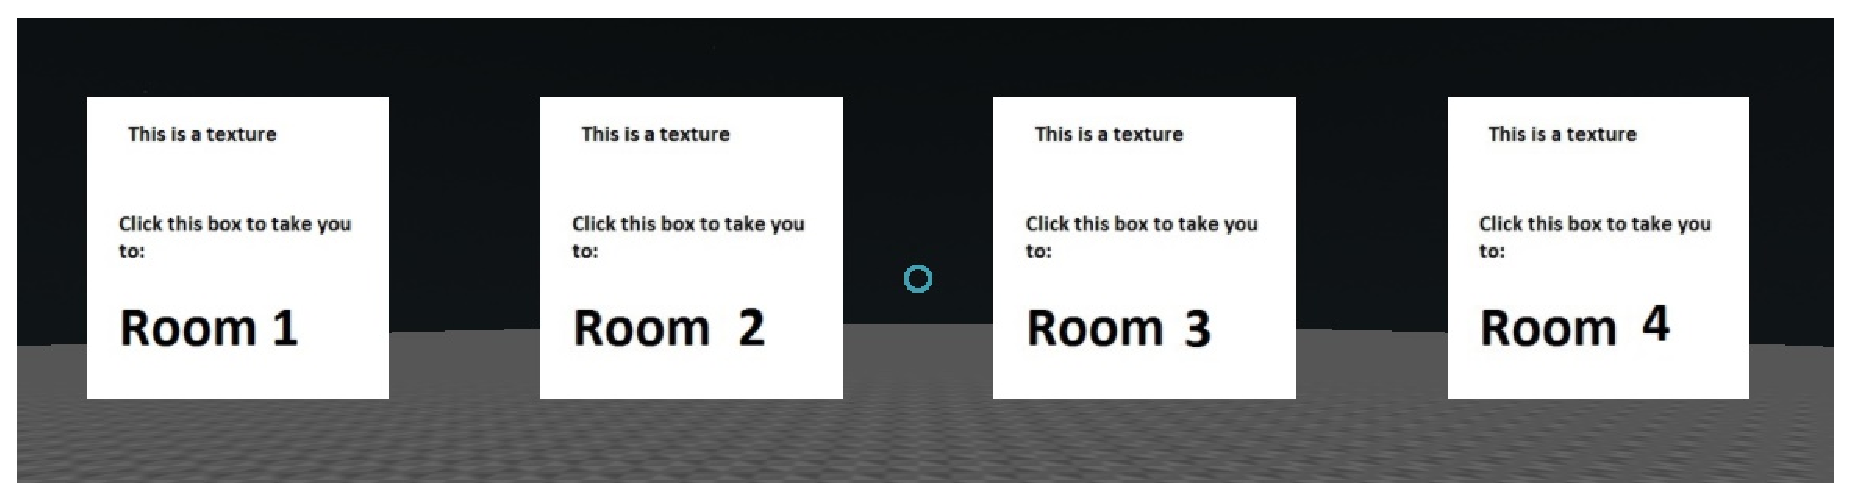
\includegraphics[width=\textwidth]{lobby.eps}\\
\textbf{Figure 1. } The lobby with four traversal links to new rooms.\\
\vspace{.75cm}
\includegraphics[width=\textwidth]{room1.eps}\\
\textbf{Figure 2. } Room 1 with multiple trees scattered in the scene.\\
\vspace{.75cm}
\includegraphics[width=\textwidth]{room2.eps}\\
\textbf{Figure 3. } Room 2 demonstrating some animations (it actually is animated).\\
\vspace{.75cm}
\includegraphics[width=\textwidth]{room3.eps}\\
\textbf{Figure 4. } Room 3 has some specific user interactions when hovering over the spheres. \\
\vspace{.75cm}
\includegraphics[width=\textwidth]{room4.eps}\\
\textbf{Figure 4. } Room 4 combines all aspect to put together an interesting scene. \\
\vspace{.75cm}
\end{center}
\end{singlespace}

\newpage

\begin{tabular}{ll}
\makebox[3.5in]{\hrulefill} & \makebox[1.5in]{\hrulefill}\\
Client Signature & Date\\
[4ex]% adds space between the two sets of signatures
\makebox[3.5in]{\hrulefill} & \makebox[1.5in]{\hrulefill}\\
Group Signature & Date\\
[4ex]% adds space between the two sets of signatures
\makebox[3.5in]{\hrulefill} & \makebox[1.5in]{\hrulefill}\\
Group Signature & Date\\
[4ex]% adds space between the two sets of signatures
\makebox[3.5in]{\hrulefill} & \makebox[1.5in]{\hrulefill}\\
Group Signature & Date\\
\end{tabular}

\end{document}
